\documentclass[final,table,14pt,svgnames]{beamer}
\usepackage[orientation=landscape,size=a4,scale=4]{beamerposter}
\setbeamertemplate{navigation symbols}{}
\usepackage{graphicx}
\usepackage{tikz}
\usepackage{marvosym}
\usepackage{pgfpages}
\usepackage{hyperref}
\usepackage{fontawesome}
\usepackage{xcolor}
\usepackage{stackengine}
\usepackage{mathdesign}
\usepackage[most]{tcolorbox}
\usetikzlibrary{calc}
\usepackage{adjustbox}
\usepackage[none]{hyphenat}
%\usefonttheme{serif}
\urlstyle{sf}
\tcbuselibrary{skins,breakable}

\AtBeginEnvironment{tcolorbox}{\tiny}


\tikzstyle{na} = [baseline=-.5ex]
\usetikzlibrary{arrows,shapes,backgrounds}
\tikzstyle{every picture}+=[remember picture]
\usetikzlibrary{spy}

\newfontfamily\titletext[Path = /home/ctroupin/.fonts/]{Aileron-Light.otf}

\usepackage{fontspec}
\defaultfontfeatures{Ligatures=TeX}
	
\definecolor{bluegher}{RGB}{4,99,128}  		% blue 
\definecolor{greygher}{RGB}{50, 50, 50}  	% grey 
\definecolor{greytext}{RGB}{100, 100, 100}  	% grey 
\definecolor{redgher}{RGB}{189, 33, 5}  	% red 
\definecolor{greybackground}{RGB}{235, 235, 235}

\hypersetup{colorlinks,linkcolor=,urlcolor=bluegher}

\setbeamerfont{title}{size=\LARGE,series=\titletext}
\setbeamerfont{subtitle}{size=\large}
\setbeamerfont{date}{size=\scriptsize}
\setbeamerfont{projected text}{size=\normalsize,series=\titletext}

\setbeamercolor{title}{fg=black}
\setbeamercolor{projected text}{fg=bluegher}
\setbeamercolor{subtitle}{bg=bluegher,fg=white}
\setbeamercolor{projected text}{fg=bluegher,bg=white}

\makeatletter
\newcommand{\srcsize}{\@setfontsize{\srcsize}{5pt}{5pt}}
\makeatother

% ------------------------------------------------
% LENGTH DEFINITIONS
%-------------------------------------------------
%\setlength{\textwidth}{24cm}
%\setlength{\textheight}{28cm}
\setbeamersize{text margin left=10pt,text margin right=10pt}

\newsavebox{\ximagebox}
\newlength{\ximageheight}
\newsavebox{\xglyphbox}
\newlength{\xglyphheight}
\newcommand{\xbox}[1]%
   {\savebox{\ximagebox}{#1}%
    \settoheight{\ximageheight}{\usebox{\ximagebox}}%
    \savebox{\xglyphbox}{\char32}%
    \settoheight{\xglyphheight}{\usebox{\xglyphbox}}%
    \raisebox{\ximageheight}[0pt][0pt]{\raisebox{-\xglyphheight}[0pt][0pt]{%
      \makebox[0pt][l]{\usebox{\xglyphbox}}}}%
    \usebox{\ximagebox}%
    \raisebox{0pt}[0pt][0pt]{\makebox[0pt][r]{\usebox{\xglyphbox}}}}
    


\newcommand{\seplogo}{\hspace{.45cm}}
\newcommand{\figheight}{.0625\textheight}

\newtcolorbox[auto counter]{maintitle}{%
  enhanced,
  width=.5\linewidth,
  before=\bigskip,
  after=\bigskip,
  colback=white,
  fonttitle=\normalsize,
  title=Careers in Oceanography,
  arc=15pt,
  colupper=black,
  height=2.25cm,
  valign=center,
  top=-2mm,
  sharp corners,
  sidebyside,
  lower separated=true,
  rounded corners=south,
  attach boxed title to top center={yshift=-\tcboxedtitleheight/2,yshifttext=-\tcboxedtitleheight/2},
  boxed title style={%
    enhanced,
    colframe=greytext,
    colback=bluegher,
    arc=5pt
  },
  frame style={%
    left color=bluegher,
    right color=bluegher},
    colbacklower=black
}

\DeclareGraphicsExtensions{.eps,.JPG,.jpg,.pdf,.png,.PNG,.jpeg}
\graphicspath{
{./logos/},
{../figures/},
}

\parindent 0cm

\usebackgroundtemplate{
\begin{tikzpicture}
\node[anchor=south west,inner sep=0cm,opacity=0.4] (image) at (0,0) {\hspace{-.5cm}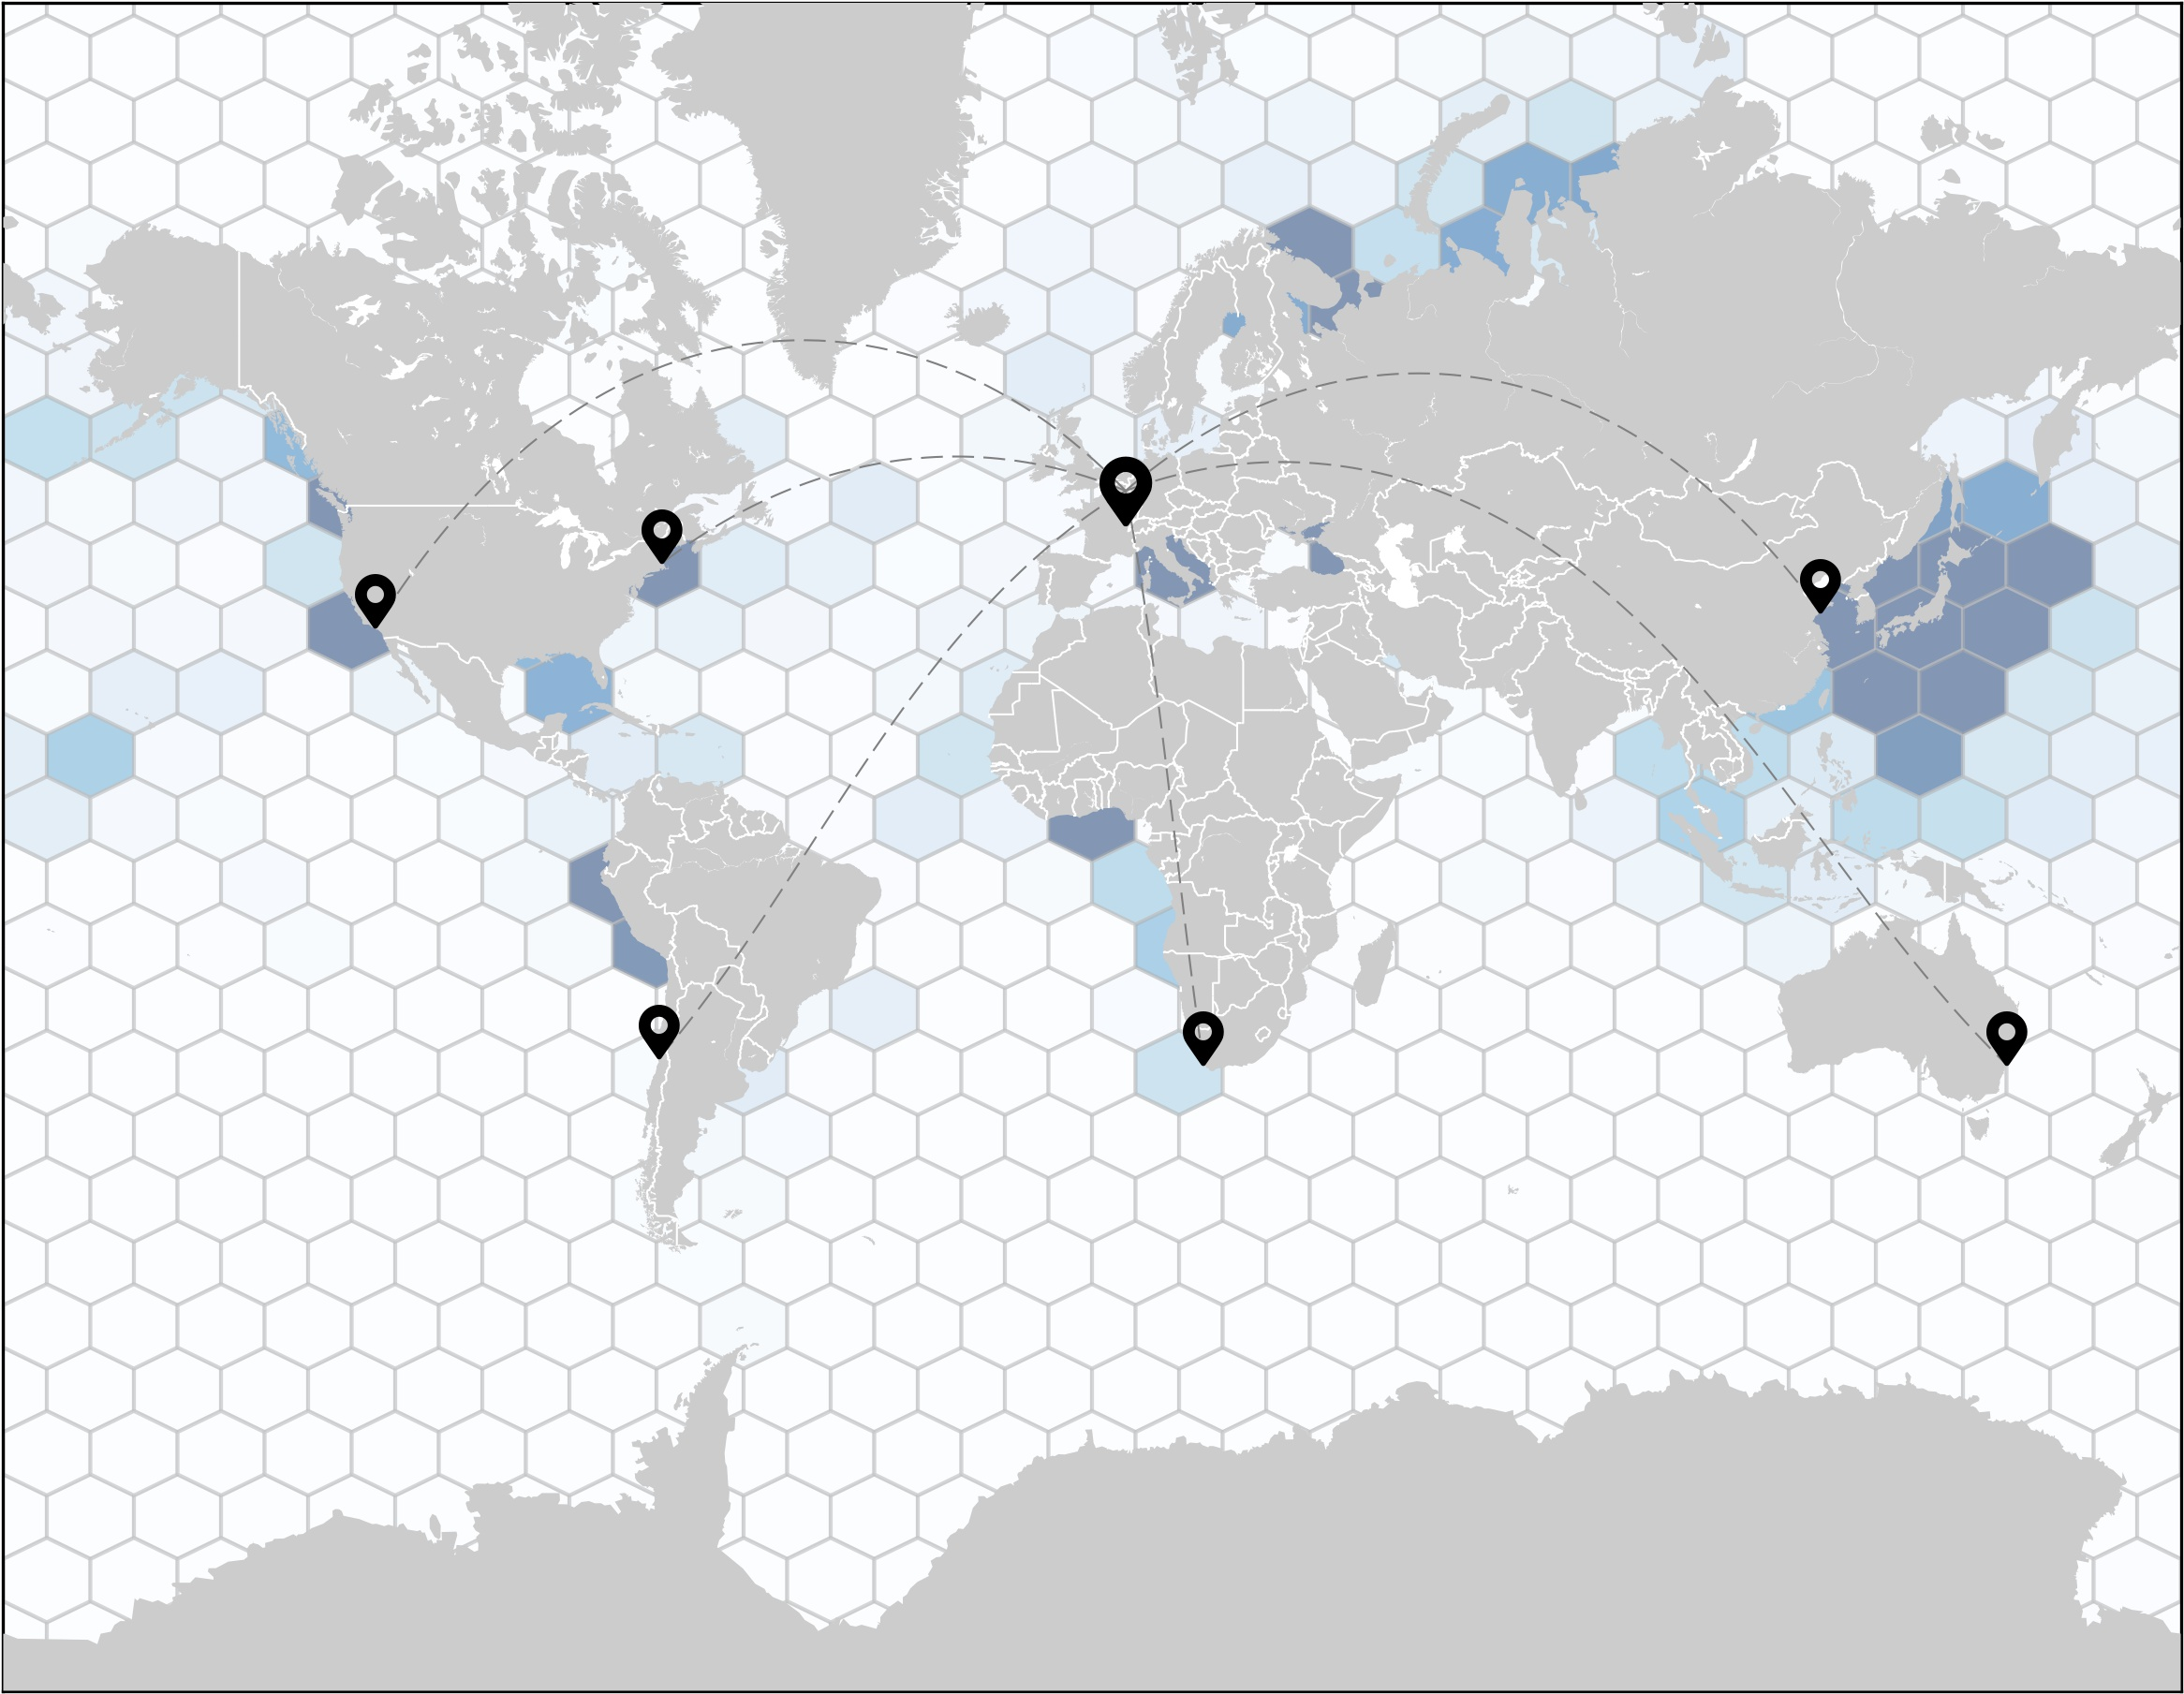
\includegraphics[width=1.05\paperwidth]{images/poster_map10.jpg}};

    \begin{scope}[x={(image.south east)},y={(image.north west)}]
    %\draw[help lines,xstep=.1,ystep=.1] (0,0) grid (1,1);
    %\foreach \x in {0,1,...,9} { \node [anchor=north] at (\x/10,0) {0.\x}; }
    %\foreach \y in {0,1,...,9} { \node [anchor=east] at (0,\y/10) {0.\y}; }
\end{scope}
\end{tikzpicture}
}
%\tikz\node[opacity=0.33]{\parbox[c][\paperheight][c]{\paperwidth}{\hspace{-.5cm}\includegraphics[width=1.05\paperwidth]{poster_map07.png}}};}

% These lines to keep good colors when viewed with Acrobat Reader
\makeatletter%
\special{pdf: put @thispage <</Group << /S /Transparency /I true /CS /DeviceRGB>> >>}%
\makeatother%

\author{}
%\url{www.socib.es}}
\title[]{Careers in Oceanography}
\date{11 December 2018, 2$-$6~PM}


\begin{document}
\def\stackalignment{l}

\begin{frame}[fragile, t]
\centering

\begin{tikzpicture}[remember picture,overlay]%

\node [anchor=south east] at (current page.south east) {\raisebox{-1cm}{\srcsize By \textsf{ctroupin}}};

\draw[line width = 2pt,dashed,bluegher] ($(current page.north west) + (1mm,-1mm)$) rectangle ($(current page.south east) + (-1mm,1mm)$);
 
\coordinate (tp1) at ([yshift=-2.5cm]current page.north west);
\coordinate (tp2) at ([yshift=-4cm]current page.north west);
\coordinate (tp3) at ([yshift=-4cm]current page.north east);
\coordinate (tp4) at ([yshift=-2.5cm]current page.north east);

\coordinate (tp5) at (current page.south west);
\coordinate (tp6) at ([yshift=2cm]current page.south west);
\coordinate (tp7) at ([yshift=2cm]current page.south east);
\coordinate (tp8) at (current page.south east);
%\filldraw[draw=bluegher,fill=bluegher,opacity=0.65] (tp1)--(tp2)--(tp3)--(tp4)--cycle;
\filldraw[draw=bluegher,fill=greybackground,opacity=0.6] (tp5)--(tp6)--(tp7)--(tp8)--cycle;

%\foreach \x in {-15,-14,...,20} { \node [anchor=north] at (\x,0) {\scriptsize \x}; }
%\foreach \y in {-20,-19,...,20} { \node [anchor=east] at (0,\y) {\scriptsize \y}; }
\node [anchor=north,opacity=0.7] at (-10,-8.) {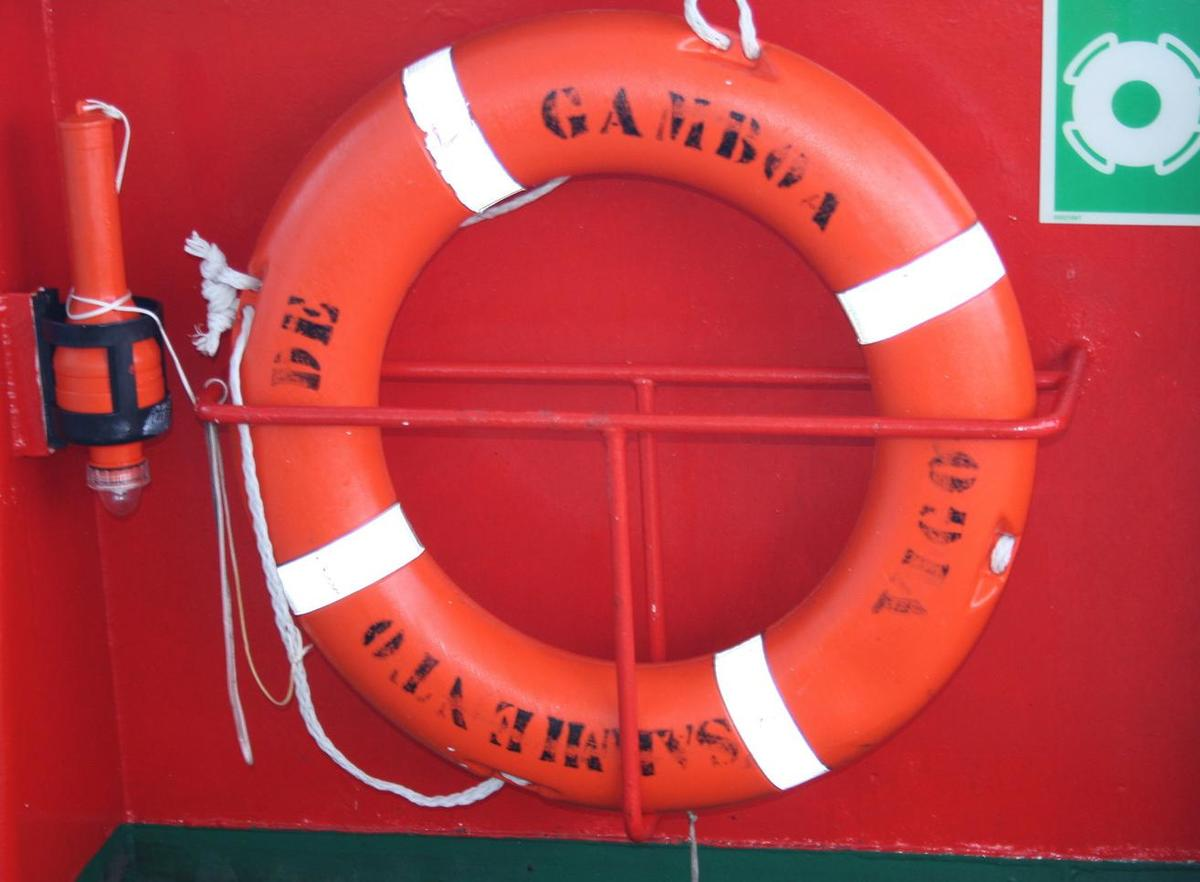
\includegraphics[width=4cm]{images/Buoy.jpg}};
\node [anchor=north,opacity=0.7] at (-6,-14.25) {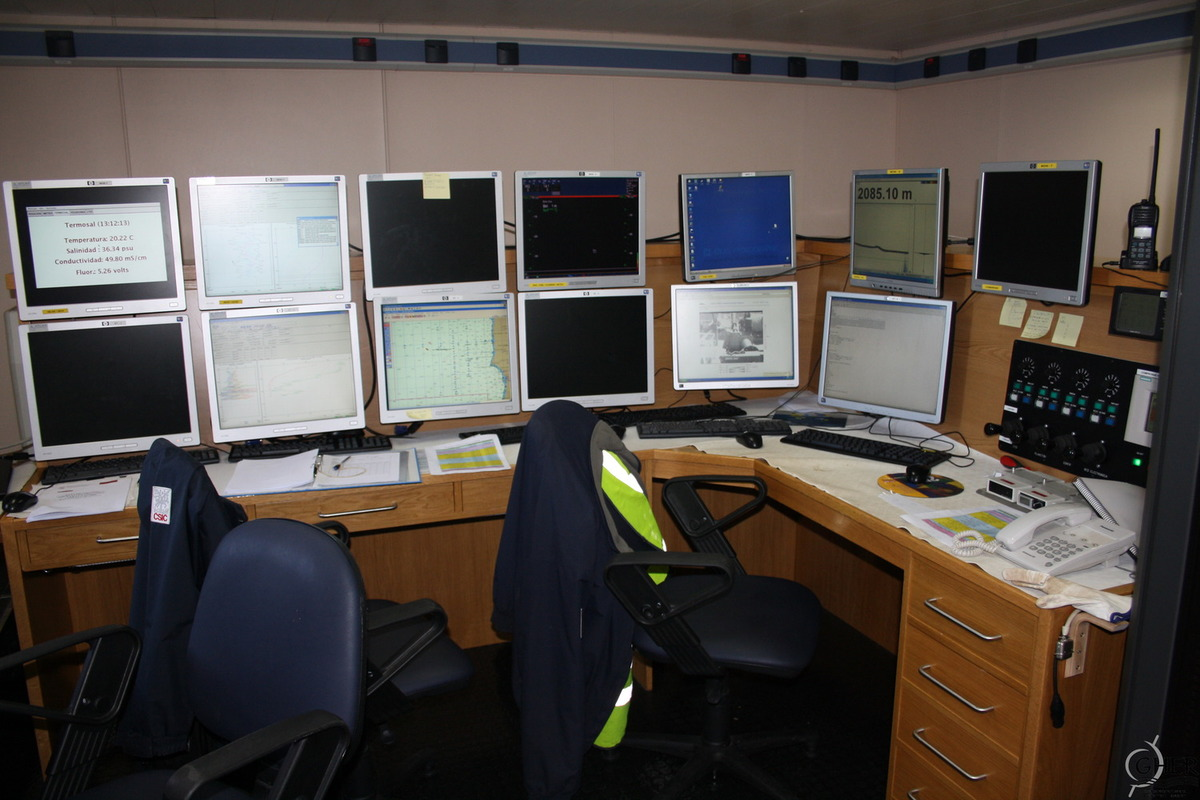
\includegraphics[width=4cm]{images/Screen.jpg}};
\node [anchor=north,opacity=0.7] at (1.8,-14.25) {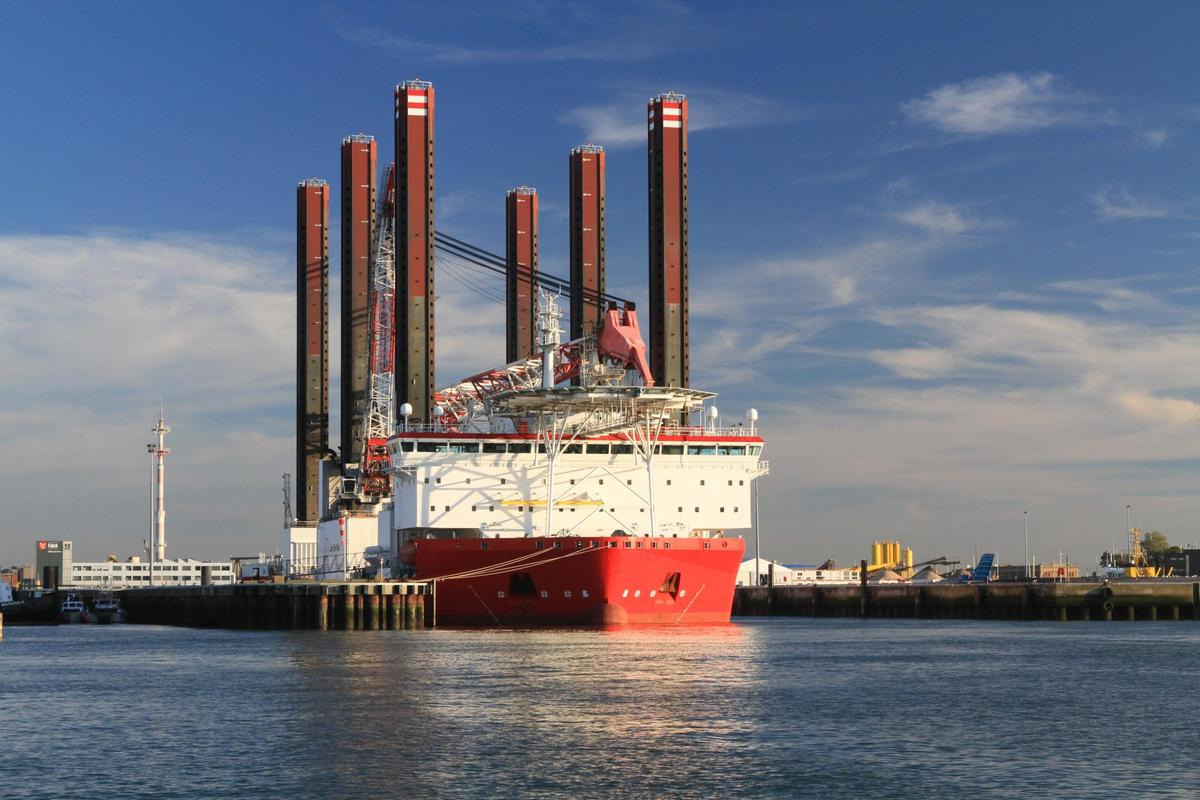
\includegraphics[width=4cm]{images/GCAN7969.JPG}};
\node [anchor=north,opacity=0.7] at (10.5,-7.5) {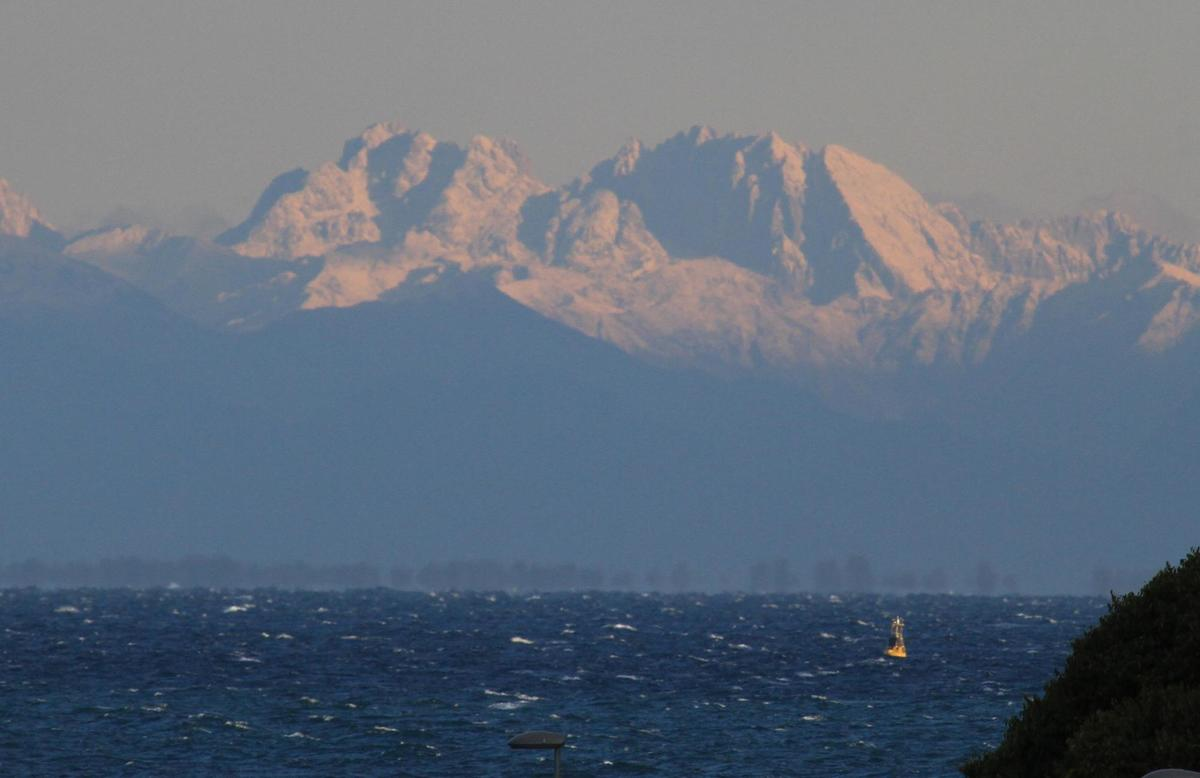
\includegraphics[width=4cm]{images/Piran2018_7802.JPG}};
\node [anchor=north east,opacity=0.7] at (13.2,-14.2) {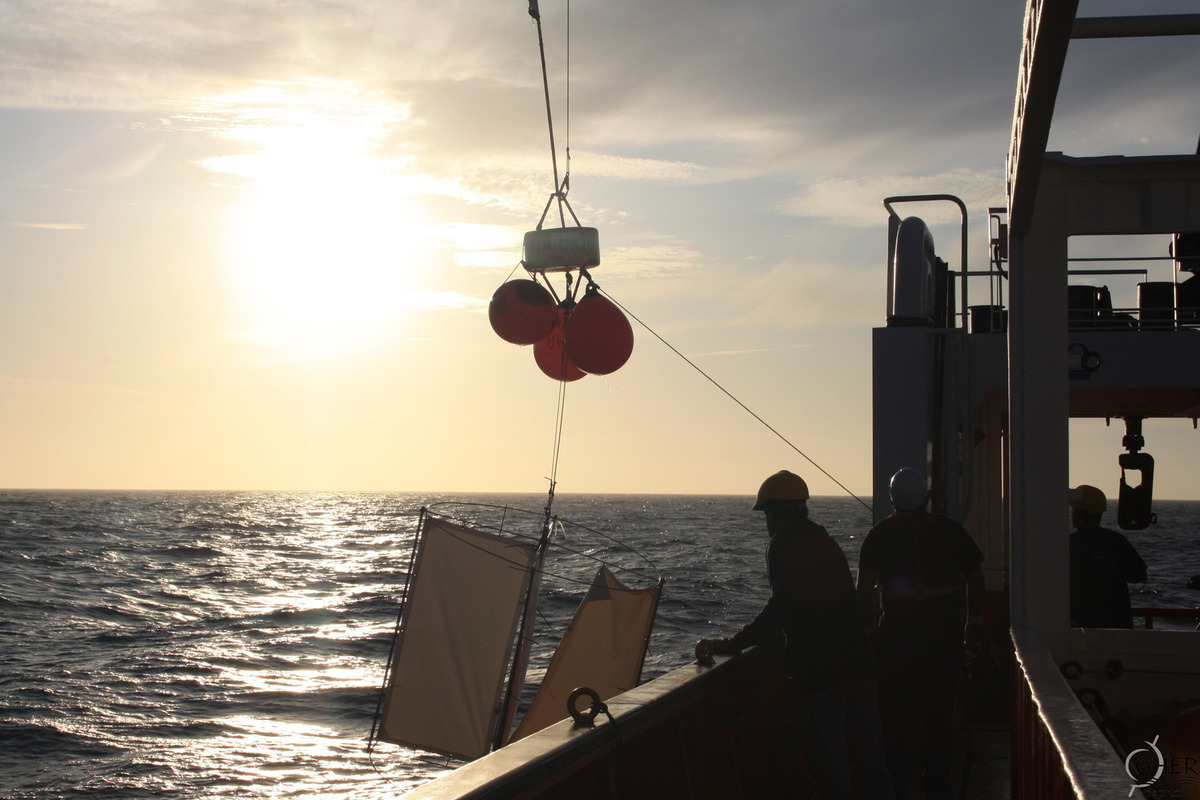
\includegraphics[width=4cm]{images/ctd.jpg}};

\end{tikzpicture}

\vspace*{1cm}

\begin{tikzpicture}[xscale=.4,yscale=.1]
\draw [bluegher,thick,smooth,domain=-5*pi:-1*pi] plot (\x, {(sin(\x r * 1.5) * (\x/2))});
\draw [greygher,thick,smooth,domain=-5*pi:-1*pi] plot (\x, { 1.5 * (sin(\x r * 1.5) * (\x/4+1))});

\end{tikzpicture}\hspace{.5cm}\begin{maintitle}
\tiny
\faMapPin~~~Exèdre Dick Annegarn \{B8\}
\tcblower
\tiny
\textcolor{greygher}{\faCalendarCheckO~~~\insertdate}
\end{maintitle}\hspace{.5cm}\begin{tikzpicture}[xscale=.4,yscale=.1]
\draw [bluegher,thick,smooth,domain=pi:5*pi] plot (\x, {(sin(\x r * 1.5) * (\x/2))});
\draw [greygher,thick,smooth,domain=pi:5*pi] plot (\x, { 1.5 * (sin(\x r * 2.) * (\x/6+1))});

\end{tikzpicture}

\vspace*{3cm}


\begin{center}
\parbox{.4\textwidth}{
\scriptsize
\centering
A half-a-day event to meet and discuss with representatives from several
Belgian and international companies and institutions operating in the
domains of oceanographic and aquatic environments.

\vspace{.2cm}

Come to discover some of the job prospects that lay ahead of your diploma in Oceanography!
}
\end{center}


\vspace{.35cm}
\vfill


%-------------------------------------
% Place the logo for the sponsors here
%-------------------------------------

\vfill

\begin{tikzpicture}[remember picture,overlay]
  \node[anchor=south] at (current page.south) {
  \begin{columns}[totalwidth=1.\textwidth,c]
\column{.51\textwidth}
\scriptsize


\includegraphics[height=\figheight]{logo_oceano_short}\seplogo
\includegraphics[height=\figheight]{logo_mast_short}\seplogo
\includegraphics[height=\figheight]{logo_gher}

\column{.5\textwidth}
\scriptsize
\hfill \stackanchor{Registration: \url{https://tinyurl.com/CareersOceanULg}}{\textcolor{greygher}{\faTwitter~@GHER\_ULg}~~\faHashtag OceanCareer18} \hspace*{1cm} 
\end{columns}
};
\end{tikzpicture}



\end{frame}



\end{document}
